\documentclass[10pt]{article}
\usepackage{amsmath}
\usepackage{tikz}
\usetikzlibrary{arrows,calc}
\begin{document}
%
\section{Constant Strain Triangle (2D)}
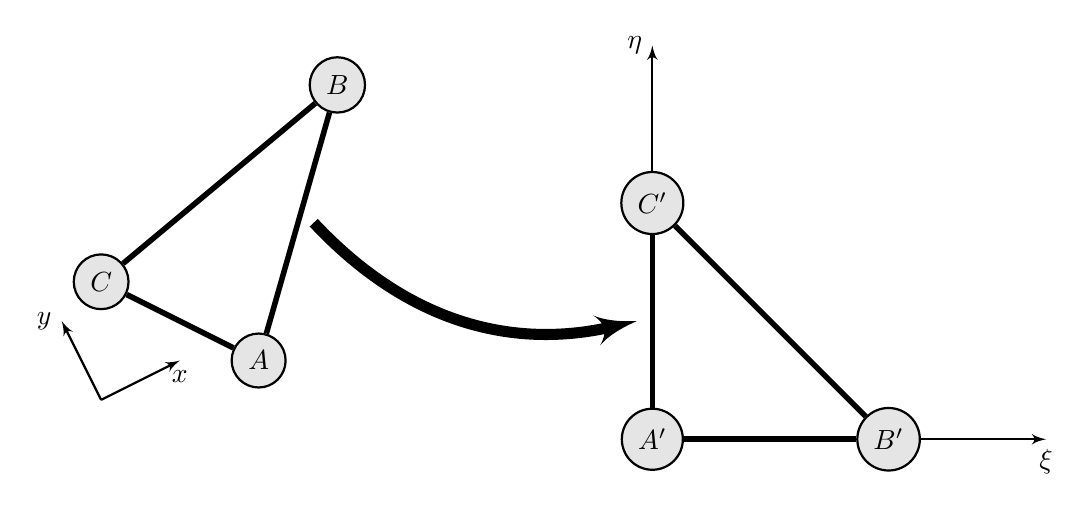
\begin{tikzpicture}[>=latex',thick]
    \tikzstyle{n}=[circle, draw=black, minimum size=0.5cm, fill=black!10]

    \node[n] (Ao) at (-5cm, 1cm) {$A$};
    \node[n] (Co) at (-7cm, 2cm) {$C$};
    \node[n] (Bo) at (-4cm, 4.5cm) {$B$};
    \draw (Ao) edge[line width=2pt] (Bo);
    \draw (Ao) edge[line width=2pt] (Co);
    \draw (Bo) edge[line width=2pt] (Co);

    \draw (-7cm, 0.5cm) edge[->] node[pos=1.0, below] {$x$} (-6cm, 1cm);
    \draw (-7cm, 0.5cm) edge[->] node[pos=1.0, left] {$y$} (-7.5cm, 1.5cm);

    \coordinate (Xm) at (5cm, 0);
    \coordinate (Ym) at (0, 5cm);
    \coordinate (xi) at (3cm, 0);
    \coordinate (eta) at (0, 3cm);
    \coordinate (origin) at (0,0);

    \coordinate (Yhalf) at ($ 0.5*(eta) + 0.5*(origin) $);

    \draw ($0.5*(Ao) + 0.5*(Bo) + (0.2cm,0)$) edge[bend right, ->,line width=4pt] ($(Yhalf) + (-0.2cm, 0)$);

    \node[n] (B) at (xi) {$B'$};
    \node[n] (C) at (eta) {$C'$};
    \node[n] (A) at (origin) {$A'$};

    \draw (A) edge[line width=2pt] (B);
    \draw (B) edge[->] node[pos=1.0, below] {$\xi$} (Xm);
    \draw (A) edge[line width=2pt] (C);
    \draw (C) edge[->] node[pos=1.0, left] {$\eta$} (Ym);
    \draw (B) edge[line width=2pt] (C);
\end{tikzpicture}

\begin{itemize}
    \item Local to global coordinates:
        \begin{align}
            \begin{bmatrix}
                x \\
                y \\
                1
            \end{bmatrix}
            &=
            \begin{bmatrix}
                A_x & B_x & C_x \\
                A_y & B_y & C_y \\
                1 & 1 & 1
            \end{bmatrix} 
            \begin{bmatrix}
                N_A \\
                N_B \\
                N_C
            \end{bmatrix} \\
            \begin{bmatrix}
                x \\
                y 
            \end{bmatrix}
            &=
            \begin{bmatrix}
                A_x & B_x & C_x \\
                A_y & B_y & C_y
            \end{bmatrix} 
            \begin{bmatrix}
                1 - \xi - \eta \\
                \xi \\
                \eta
            \end{bmatrix} \\
            \begin{bmatrix}
                x \\
                y 
            \end{bmatrix}
            &=
            \begin{bmatrix}
                A_x \\
                A_y 
            \end{bmatrix}
            +
            \begin{bmatrix}
                B_x - A_x & C_x - A_x \\
                B_y - A_y & C_y - A_y
            \end{bmatrix} 
            \begin{bmatrix}
                \xi \\
                \eta
            \end{bmatrix}
        \end{align}
    \item Jacobian:
        \begin{align}
            \mathbf{J} &= \frac{\partial \mathbf{x}}{\partial \boldsymbol{\xi}}
            =
            \begin{bmatrix}
                \frac{\partial x}{\partial \xi} & \frac{\partial x}{\partial \xi} \\
                \frac{\partial y}{\partial \eta} & \frac{\partial y}{\partial \eta}
            \end{bmatrix}
            =
            \begin{bmatrix}
                B_x - A_x & C_x - A_x \\
                B_y - A_y & C_y - A_y
            \end{bmatrix} \\
            \det \mathbf{J}
            &= (B_x - A_x)(C_y - A_y) - (B_y - A_y)(C_x - A_x)
        \end{align}
    \item Shape functions:
        \begin{align}
            \mathbf{N}
            &=
            \begin{bmatrix}
                N_A \\
                N_B \\
                N_C
            \end{bmatrix}
            =
            \begin{bmatrix}
                1- \xi - \eta \\
                \xi \\
                \eta
            \end{bmatrix}
        \end{align}
    \item Gradient of shape functions:
        \begin{align}
            \frac{\partial \mathbf{N}}{\partial \mathbf{x}}
            &=
            \begin{bmatrix}
                \frac{\partial N_A}{\partial x} & \frac{\partial N_A}{\partial y} \\
                \frac{\partial N_B}{\partial x} & \frac{\partial N_B}{\partial y} \\
                \frac{\partial N_C}{\partial x} & \frac{\partial N_C}{\partial y}
            \end{bmatrix}
            =
            \begin{bmatrix}
                \frac{\partial N_A}{\partial \xi} & \frac{\partial N_A}{\partial \eta} \\
                \frac{\partial N_B}{\partial \xi} & \frac{\partial N_B}{\partial \eta} \\
                \frac{\partial N_C}{\partial \xi} & \frac{\partial N_C}{\partial \eta}
            \end{bmatrix}
            \begin{bmatrix}
                \frac{\partial \xi}{\partial x} & \frac{\partial \xi}{\partial y} \\
                \frac{\partial \eta}{\partial x} & \frac{\partial \eta}{\partial y}
            \end{bmatrix} \\
            \frac{\partial \mathbf{N}}{\partial \mathbf{x}}
            &=
            \frac{1}{\det \mathbf{J}}
            \begin{bmatrix}
                -1 & -1 \\
                1 & 0 \\
                0 & 1
            \end{bmatrix}
            \begin{bmatrix}
                C_y - A_y & -(C_x - A_x) \\
                -(B_y - A_y) & B_x - A_x
            \end{bmatrix} \\
            \frac{\partial \mathbf{N}}{\partial \mathbf{x}}
            &=
            \frac{1}{\det \mathbf{J}}
            \begin{bmatrix}
                B_y - C_y & C_x - B_x \\
                C_y - A_y & A_x - C_x \\
                A_y - B_y & B_x - A_x
            \end{bmatrix}
        \end{align}
\end{itemize}

\end{document}
